\section{Finding optimal bandwidth}

\subsection{Part 1}
\subsubsection{Part (a)}

We know that the estimator for distribution function $\hat{f}$ is given by

\begin{equation}
    \hat{f}(x) = \sum_{j=1}^m \frac{\hat{p}_j}{h} \mathbbm{1}\left[x \in B_j\right]
\end{equation}

\hspace{-14pt}Also given, $v_j$ is the number of points falling in the $j^{th}$ bin and $\hat{p}_j = \frac{v_j}{n}$. Using this we get,

\begin{align*}
    \int \hat{f}(x)^2 dx &= \int \left(\sum_{j=1}^m \frac{\hat{p}_j}{h} \mathbbm{1}\left[x \in B_j\right]\right)^2 dx \\
    &= \sum_{i=1}^m \int_{B_i} \left(\sum_{j=1}^m \frac{\hat{p}_j}{h} \mathbbm{1}\left[x \in B_j\right]\right)^2 dx &\text{(Segmenting the interval over the bins)}\\
    &= \sum_{j=1}^m \int_{B_j} \left(\frac{\hat{p}_j}{h}\right)^2 dx &\text{(Only the jth interval sets the indicator function)}\\
    &= \sum_{i=1}^m \left(\frac{\hat{p}_j}{h}\right)^2 \times h &\text{(Width of each bin is h)}\\
    &= \frac{1}{n^2h} \sum_{j=1}^m v_j^2
\end{align*}

\subsubsection{Part (b)}

The histogram estimator after removing the $i^{th}$ observation is given by

\begin{equation}
    \hat{f}_{(-i)}(x) = \sum_{j=1}^m \frac{\hat{p}_{j, -i}}{h} \mathbbm{1}\left[x \in B_j\right]
\end{equation}

\hspace{-19pt} where $\hat{p}_{j, -i} = \frac{v_{j, -i}}{n-1}$ and $v_{j, -i}$ is the number of points falling in the $j^{th}$ bin after removing the $i^{th}$ observation. Now, 

\begin{align*}
    \sum_{i=1}^n \hat{f}_{(-i)}(X_i) &= \sum_{i=1}^n \sum_{j=1}^m \frac{\hat{p}_{j, -i}}{h} \mathbbm{1}\left[X_i \in B_j\right] \\
    &= \sum_{i=1}^n\sum_{j=1}^m \frac{v_{j, -i}}{(n-1)h} \mathbbm{1}\left[X_i \in B_j\right] \\
    &= \sum_{j=1}^m \sum_{i=1}^n \frac{v_{j, -i}}{(n-1)h} \mathbbm{1}\left[X_i \in B_j\right] \\
    &= \sum_{j=1}^m \frac{v_{j}-1}{(n-1)h} \left( \sum_{i=1}^n \mathbbm{1}\left[X_i \in B_j\right]\right) & (\text{since whenever }\mathbbm{1}[X_i \in B_j] = 1, v_{j, -i} = v_j - 1 ) \\
    &= \sum_{j=1}^m \frac{v_{j} -1}{(n-1)h} v_j \\
    &= \frac{1}{(n-1)h} \sum_{j=1}^m (v_j^2 - v_j)
\end{align*}

\subsection{Part 2}

\subsubsection{Part (a)}

The histogram of the filtered data for number of bins = 10 is shown in Figure \ref{fig:q1_2_a}.

\begin{figure}[H]
    \centering
    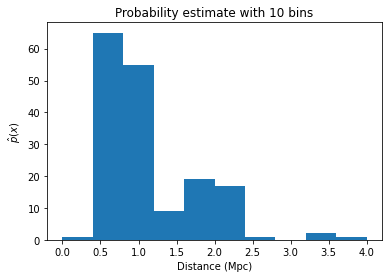
\includegraphics[width=0.5\textwidth]{../q1/images/10binhistogram.png}
    \caption{Histogram of filtered data with 10 bins}
    \label{fig:q1_2_a}
\end{figure}

The values of $\hat{p}_j$ are as follows:

\begin{tabular}
    { |c|c|c|c|c|c|c|c|c|c|c| }
    \hline
    Bin & 1 & 2 & 3 & 4 & 5 & 6 & 7 & 8 & 9 & 10 \\
    \hline
    $\hat{p}_j$ & 0.006 & 0.382 & 0.324 & 0.053 & 0.112 & 0.1 & 0.006 & 0.0 & 0.012 & 0.006 \\
    \hline
\end{tabular}

\subsubsection{Part (b)}

The probablility distribution is underfit as the number of bins is too low. The distribution is not smooth and the bins are too wide. This is evident from the histogram in Figure \ref{fig:q1_2_a}.

\subsubsection{Part (c)}

The graph of $\hat{J}(h)$ vs $h$ for the number of bins ranging from 1 to 1000 is shown in Figure \ref{fig:q1_2_c}.

% \begin{figure}[H]
%     \centering
%     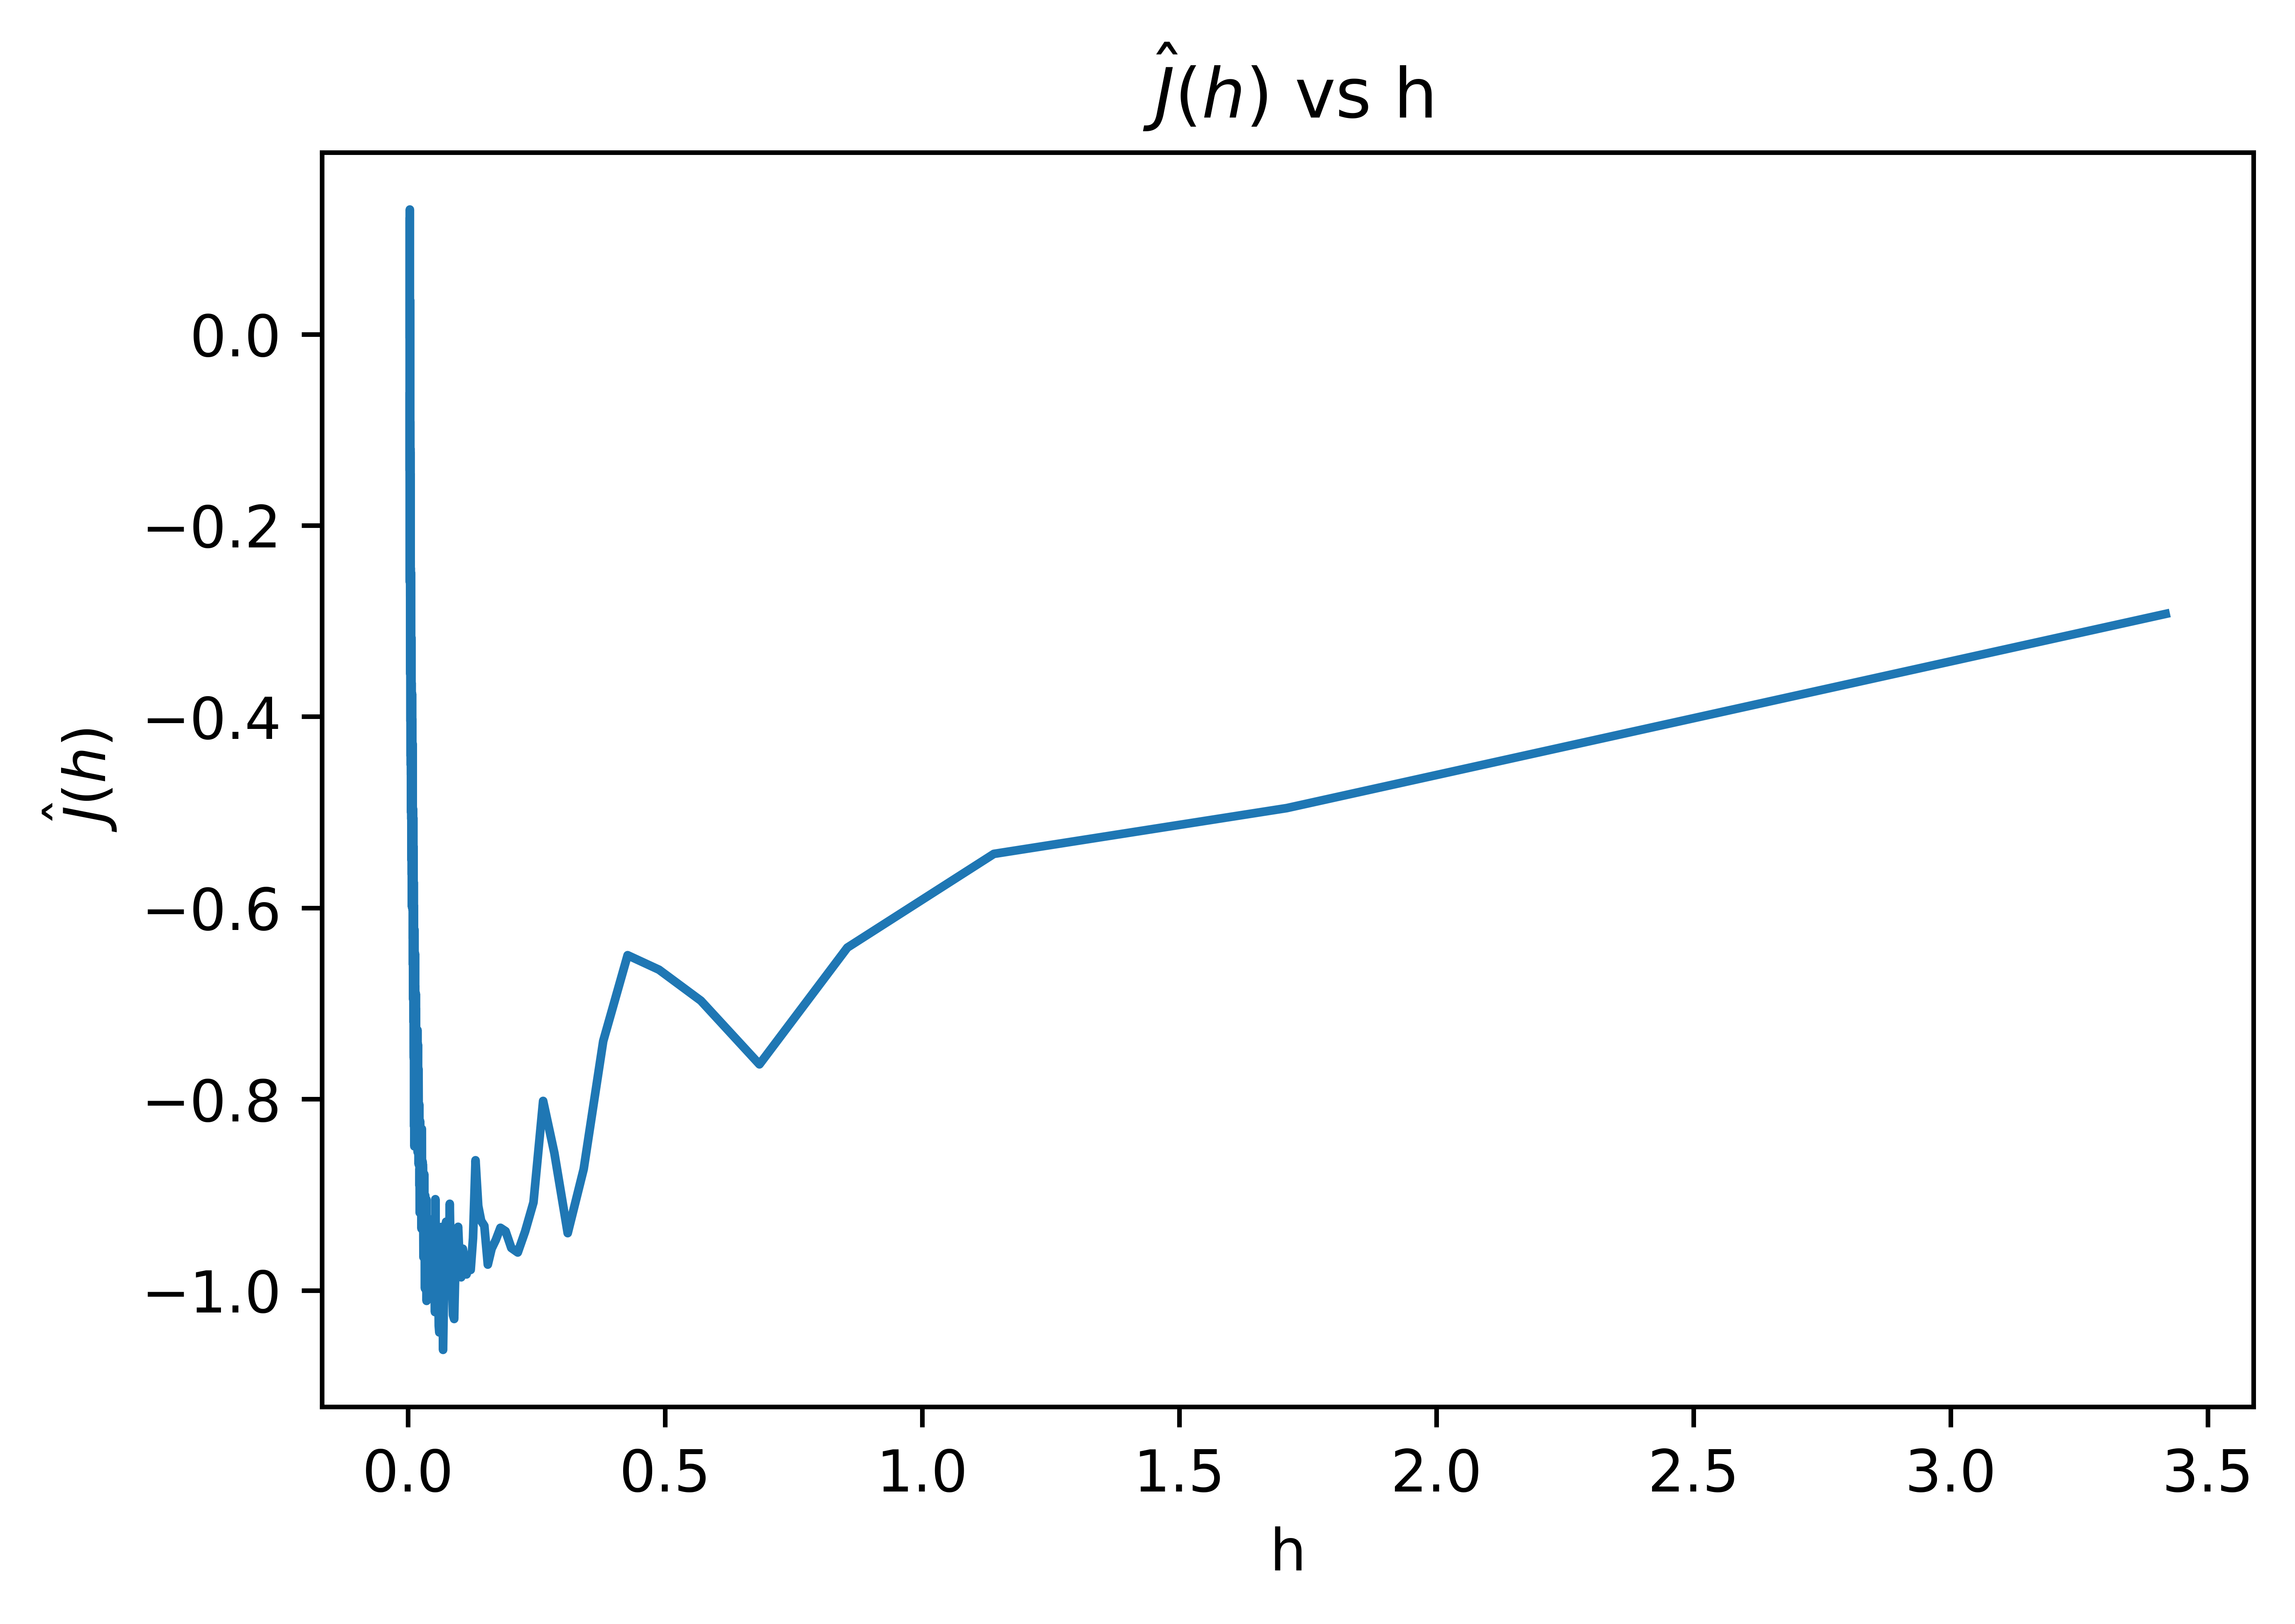
\includegraphics[width=0.5\textwidth]{../q1/images/crossvalidation.png}
%     \caption{$\hat{J}(h)$ vs $h$}
%     \label{fig:q1_2_c}
% \end{figure}

\begin{figure}
    \centering
    \begin{subfigure}{0.45\textwidth}
        \centering
        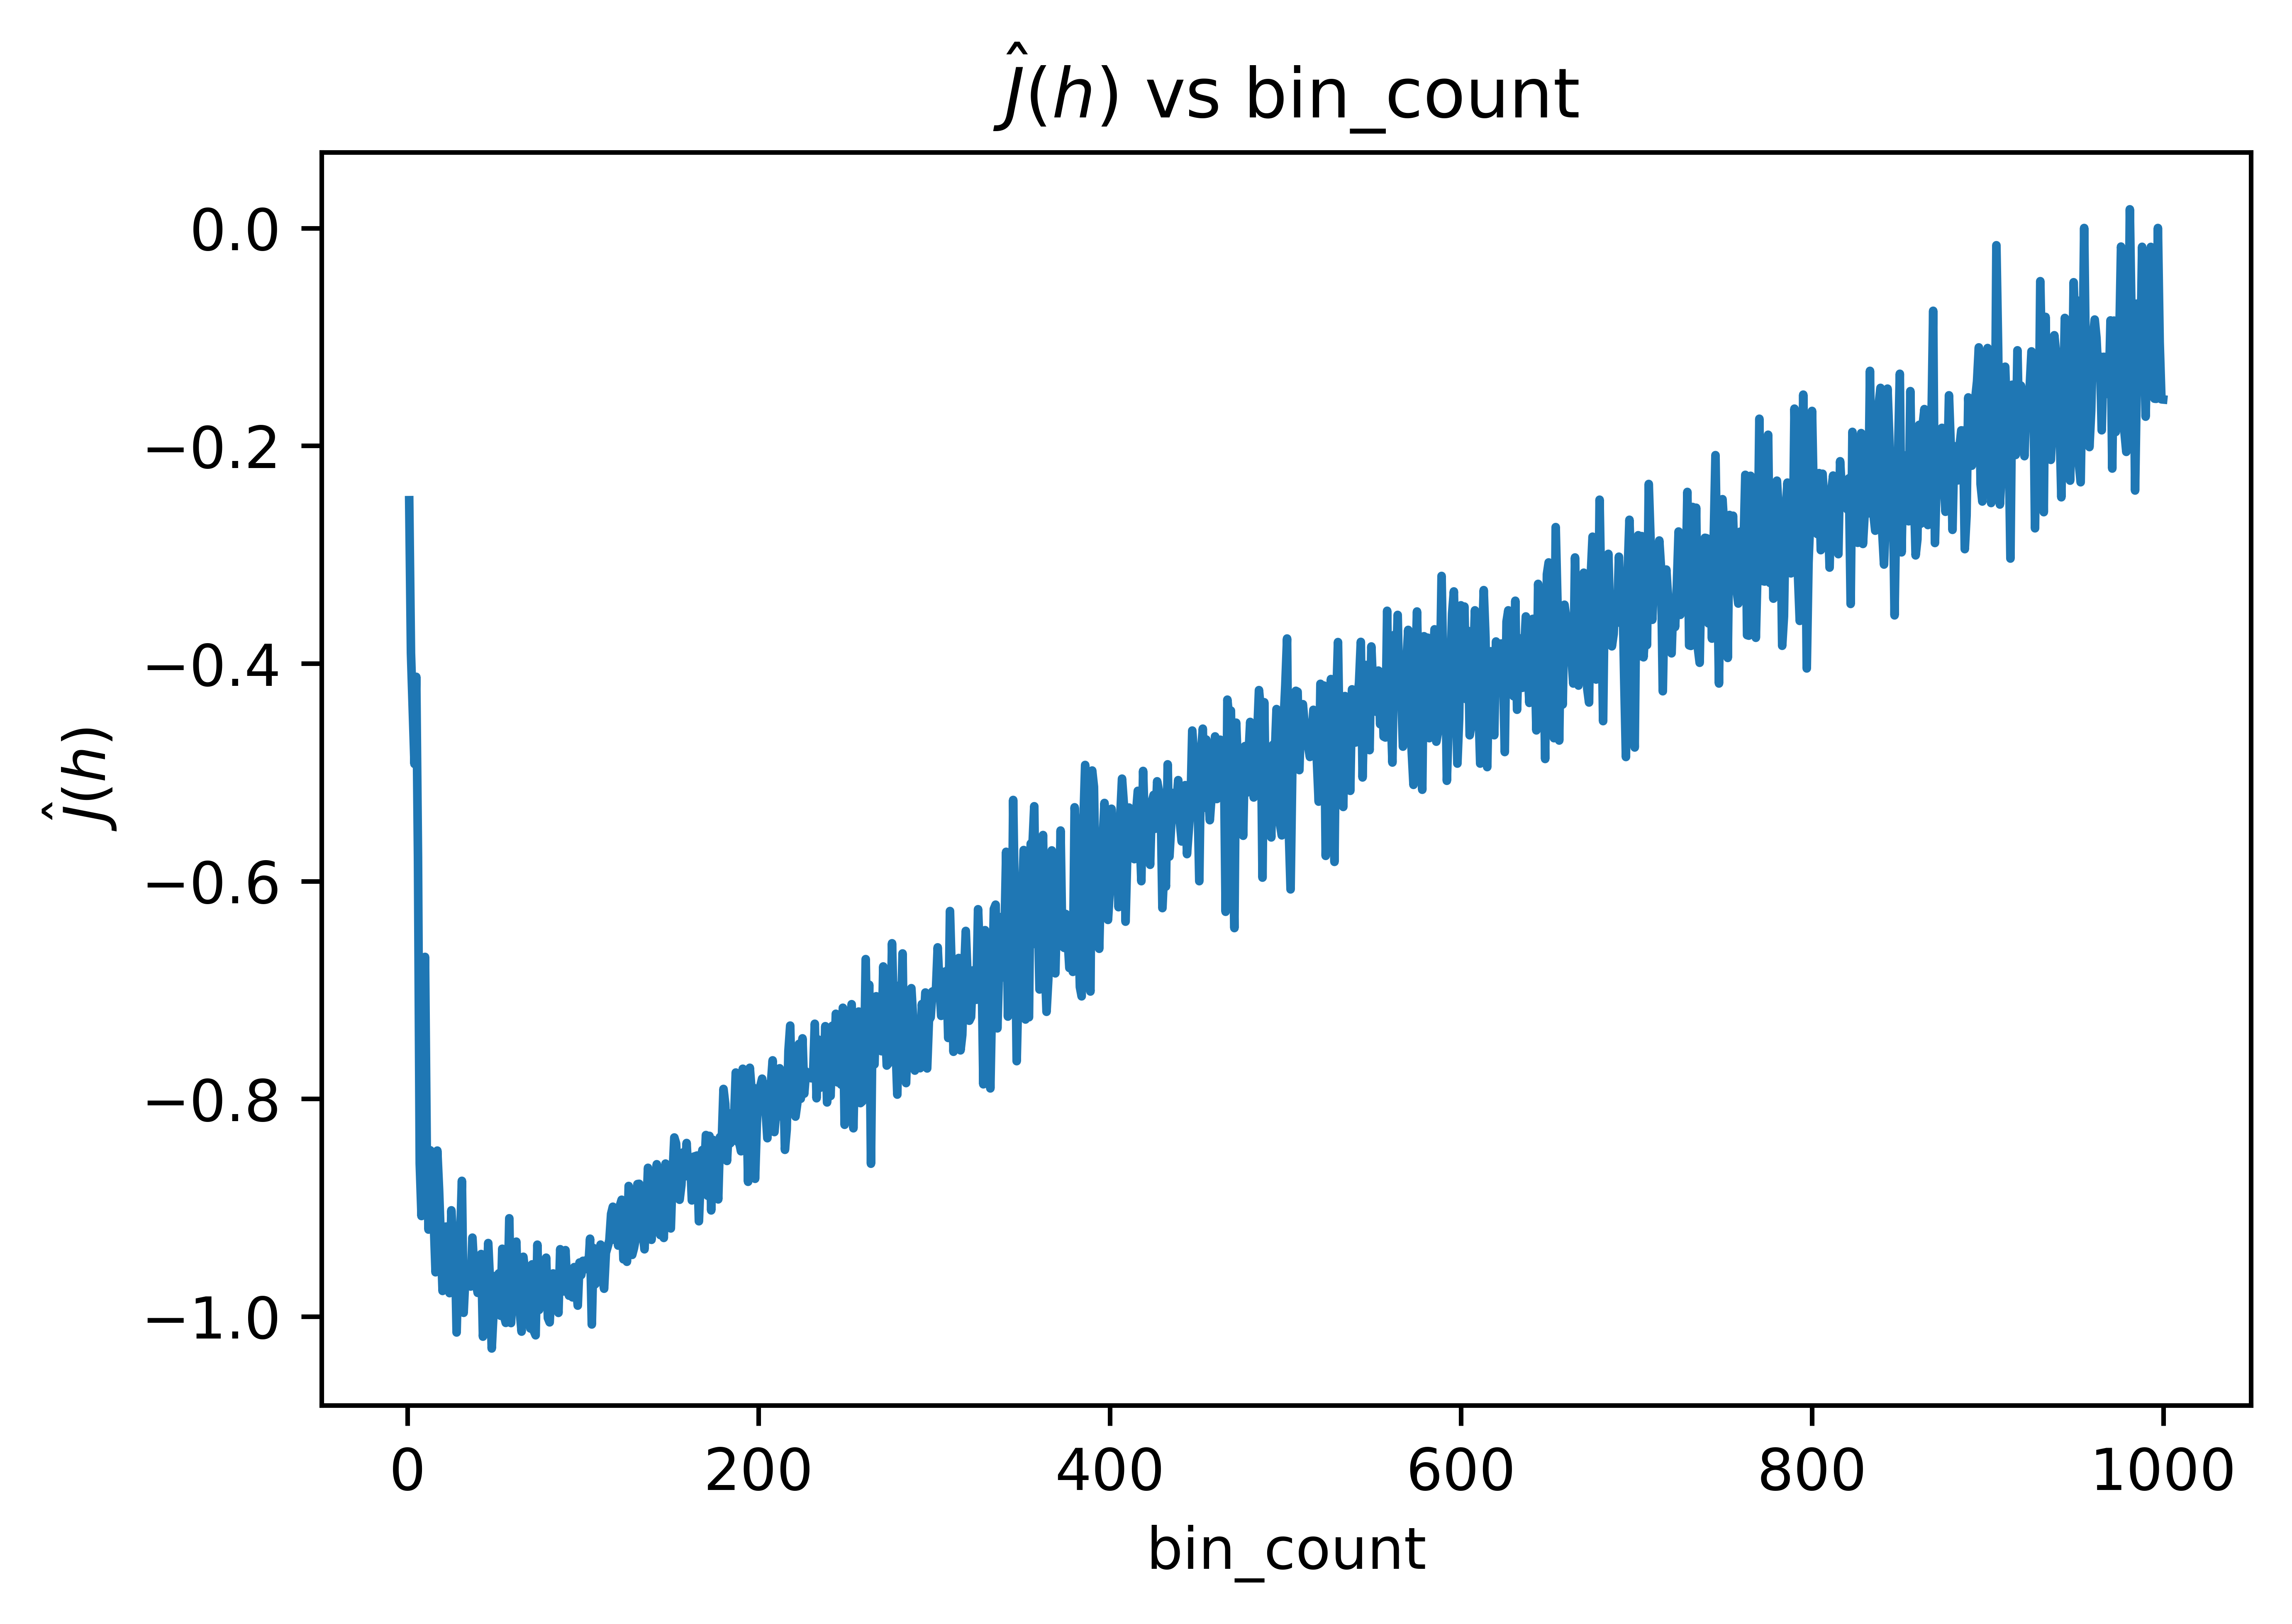
\includegraphics[width=\linewidth]{../q1/images/bins.png}
        \caption{Histogram of filtered data with 10 bins}
        \label{fig:q1_2_a}
    \end{subfigure}
    \begin{subfigure}{0.45\textwidth}
        \centering
        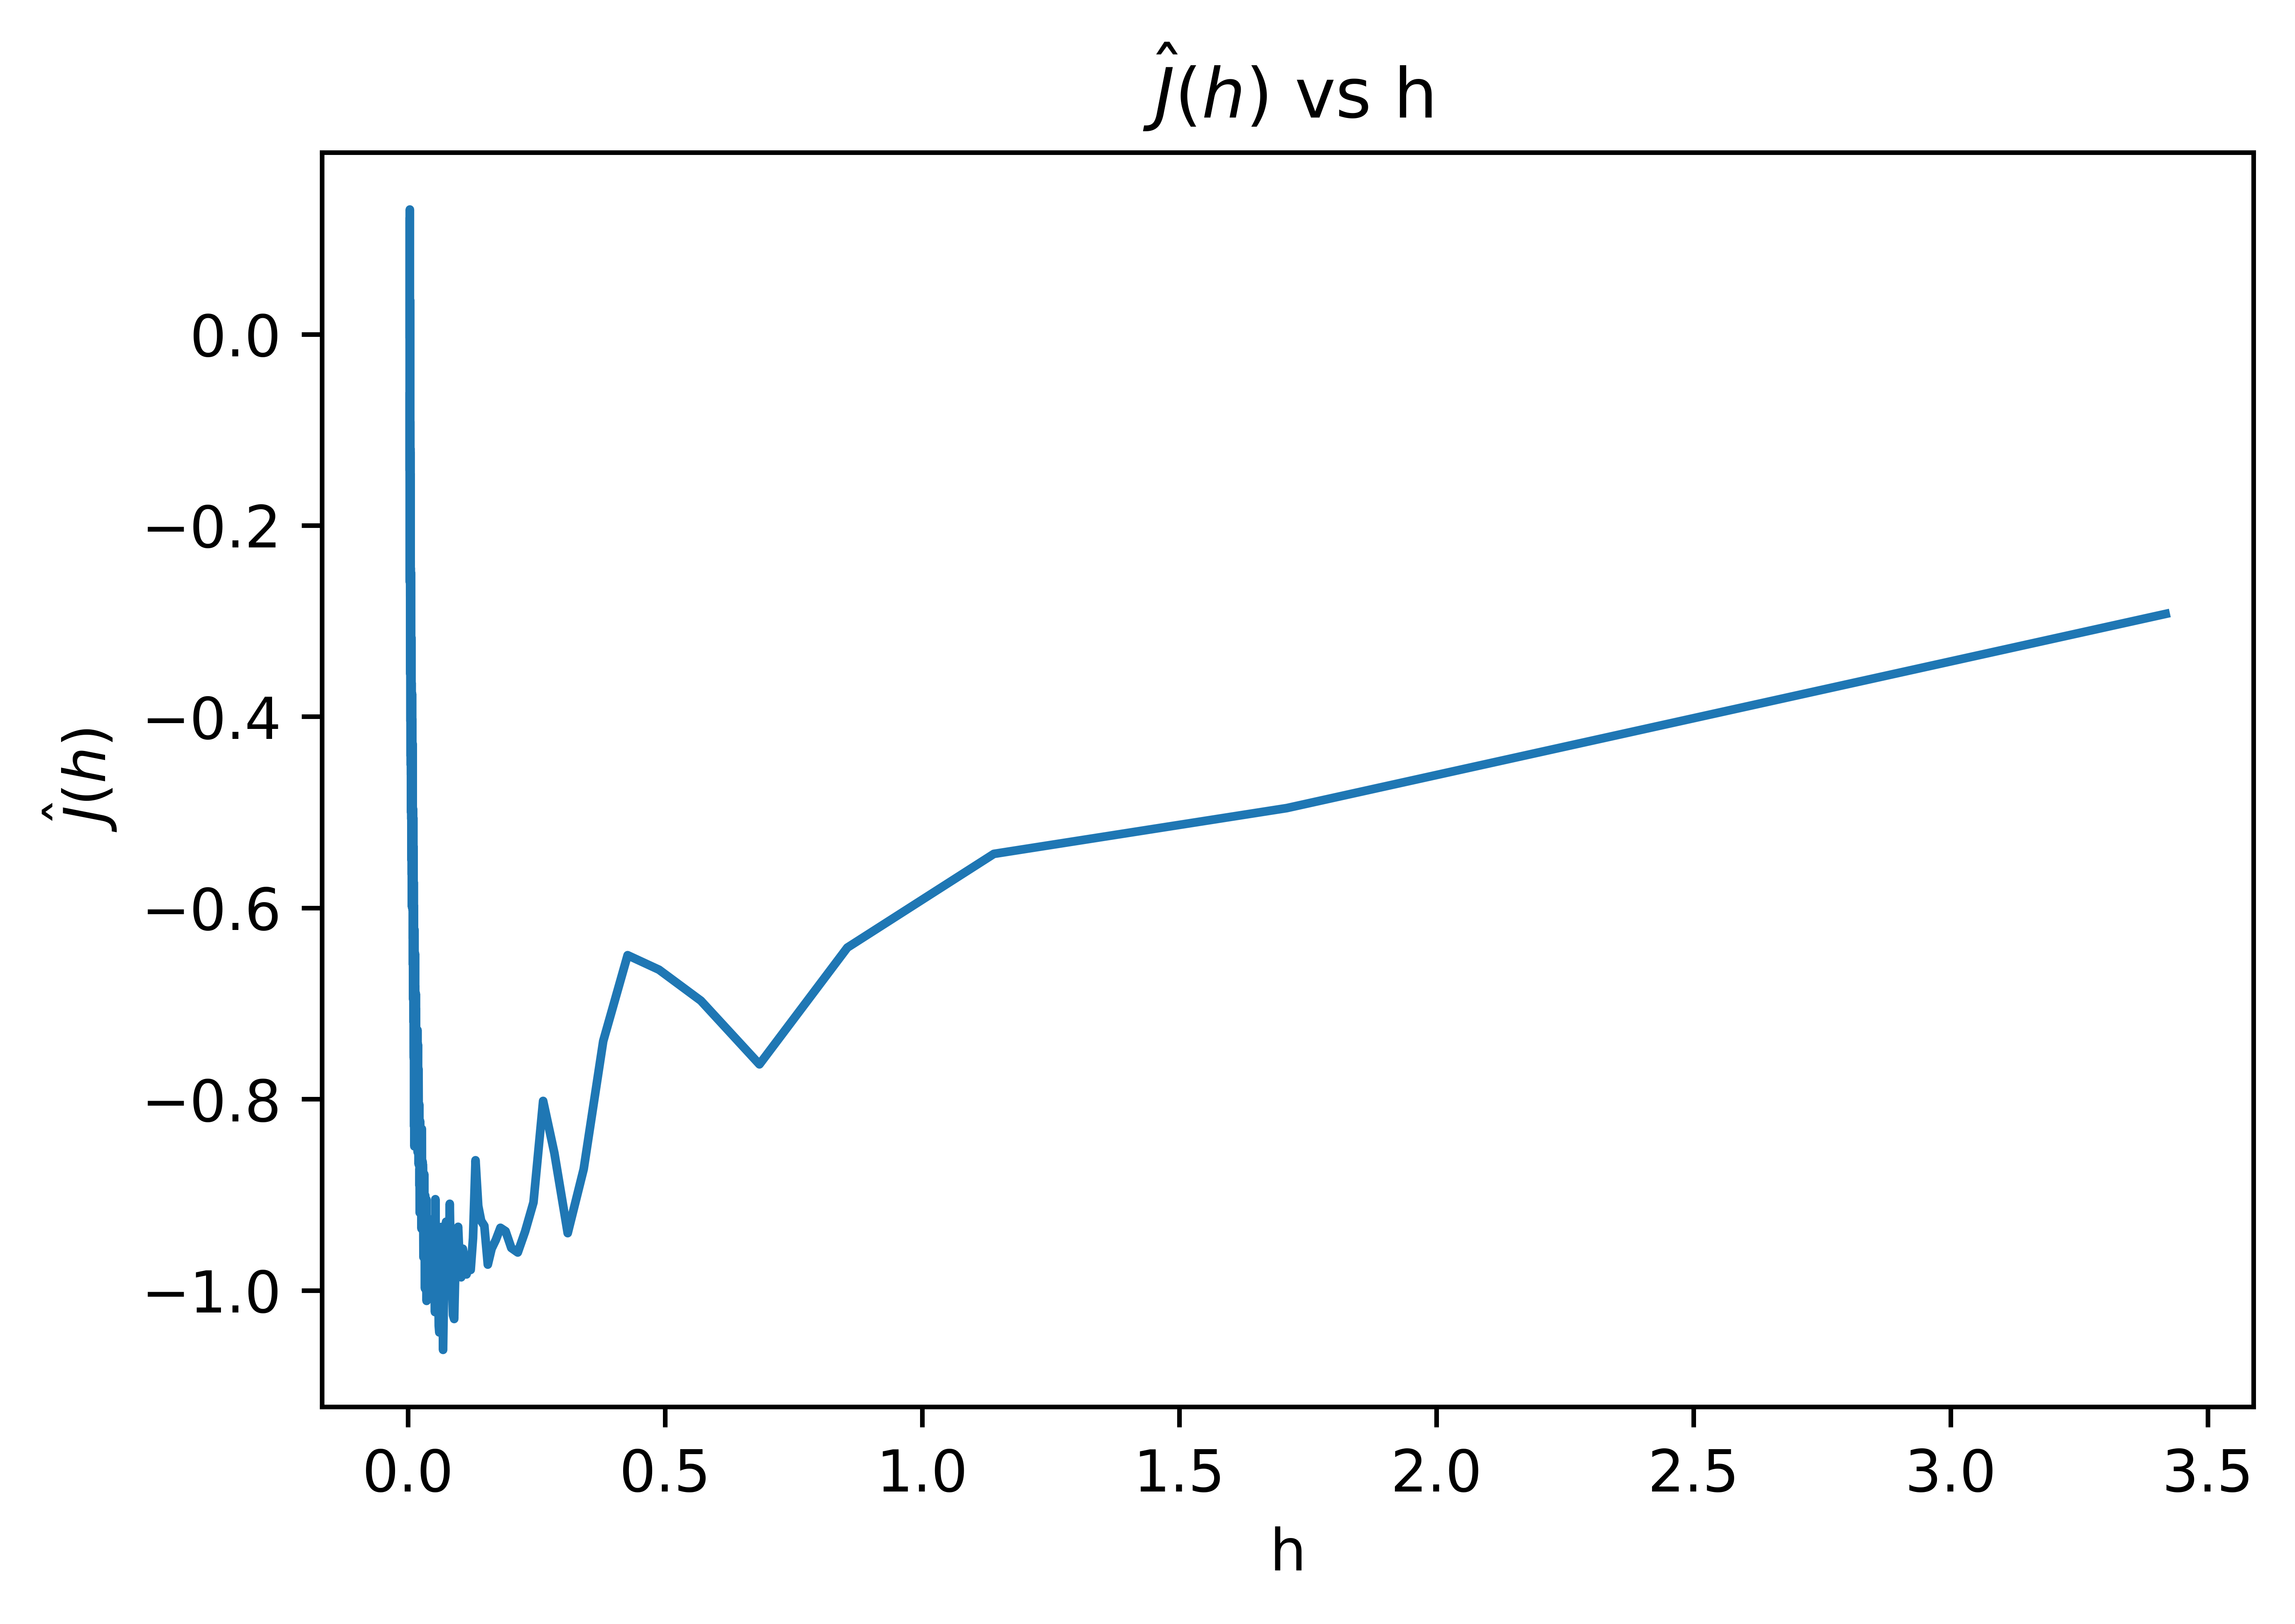
\includegraphics[width=\linewidth]{../q1/images/crossvalidation.png}
        \caption{$\hat{J}(h)$ vs $h$}
        \label{fig:q1_2_c}
    \end{subfigure}
\end{figure}

\subsubsection{Part (d)}

Based on the Cross Validation plot in Figure \ref{fig:q1_2_c}, the optimal number of bins is 48 with a value of $h^\ast = 0.0833$.

\subsubsection{Part (e)}

The histogram of the filtered data for number of bins = 48 is shown in Figure \ref{fig:q1_2_e}.

\begin{figure}[H]
    \centering
    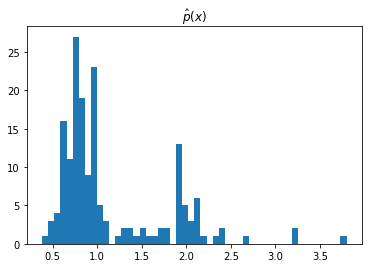
\includegraphics[width=0.45\textwidth]{../q1/images/optimalhistogram.png}
    \caption{Histogram of filtered data with 50 bins}
    \label{fig:q1_2_e}
\end{figure}

\hspace{-16pt}The graph is now just right and is neither oversmoothed nor undersmoothed. This is clearly evident when we compare the histograms in Figure \ref{fig:q1_2_a} we can realize that the data will have a higher variance leading to an overall higher risk as compared to \ref{fig:q1_2_e}.
\newpage
